\section{Testing the harness: a prospective experiment}\label{sec:experiment}

The experiment asks whether scheduled correction improves the repository
inherited by later feature work. RQ3 is addressed by the prospective design
specified below.
The 1 November amendment supersedes v4's two runs per arm/model.
Historical freezes, diagnostics and the original owner-reported OSF
registration are retained; none approves this new design. The researcher
kit requires a new source-bound freeze and prospective OSF amendment
before collection. Agent configuration
protocols and empirical-study guidance inform this pre-data design
~\cite{lulla2026protocol,baltes2026guidelines,wohlin2012experimentation}.

\subsection{Design and estimands}\label{sec:protocolsummary}

One independent replicate is a fresh repository trajectory through S1's
ten ordered features and a final held-out change request, CR1.
Every selected model, GPT~6.1 Sol, Sonnet~5.5 and Gemini~4 Argon,
runs every arm. Randomised interleaving within model/replicate blocks
uses seed 2027. Feature steps, tests and checkpoints are repeated
observations within a trajectory, not independent replicates.

\begin{table}[!htbp]
\centering\small
\caption{Prospective five-arm allocation. D is the matched-resource A+
control; E tests visible regression repair, not hidden-test feedback.}
\label{tab:protocolsummary}
\begin{tabularx}{\textwidth}{@{}L{1cm}YL{3.6cm}@{}}
\toprule
Arm & Intervention and information & Per-cycle ceilings \\
\midrule
A & Feature delivery only & 30 min; 300 nominal credits \\
B & Feature, then behaviour-preserving consolidation, additional tests
and replacement DESIGN.md & 30 + 15 min; 300 + 300 credits \\
C & Feature, then read-only review and replacement REVIEW.md
& 30 + 15 min; 300 + 300 credits \\
D (A+) & Longer feature delivery, without a scheduled consolidation pause
& 45 min; 600 credits \\
E & Feature, then repair of previously specified behaviour using visible
specifications and examples & 30 + 15 min; 300 + 300 credits \\
\bottomrule
\end{tabularx}
\end{table}

B--D is the primary practical comparison: consolidation versus giving
the builder the same total time and nominal credits. Equal ceilings do
not guarantee equal realised resources; D also has fewer fresh sessions.
B--A measures the additional package; B--C also changes editing rights,
tests and handover content. E--B contrasts visible behavioural repair with
behaviour-preserving consolidation. These secondary package comparisons
do not isolate refactoring or any of the five case mechanisms.

C cannot repair code during its review session, but REVIEW.md can direct
repairs in later feature sessions. Follow-through needs review-item and
diff locators with external adjudication; file overlap alone is not proof.
B's added tests must agree with visible specifications, rather than
legitimating a defect. Subsequent feature sessions must keep accepted
tests green. E can correct an agent-authored expectation only with a
specific contradictory specification and a retained explanation.
Accepted Python test files are immutable in full, including imports,
fixtures and module/class constants; additions use new files.
E retains only its explicit specification-bound correction exception.
Immutable example tests remain protected in every arm.

\begin{figure}[!htbp]
\centering
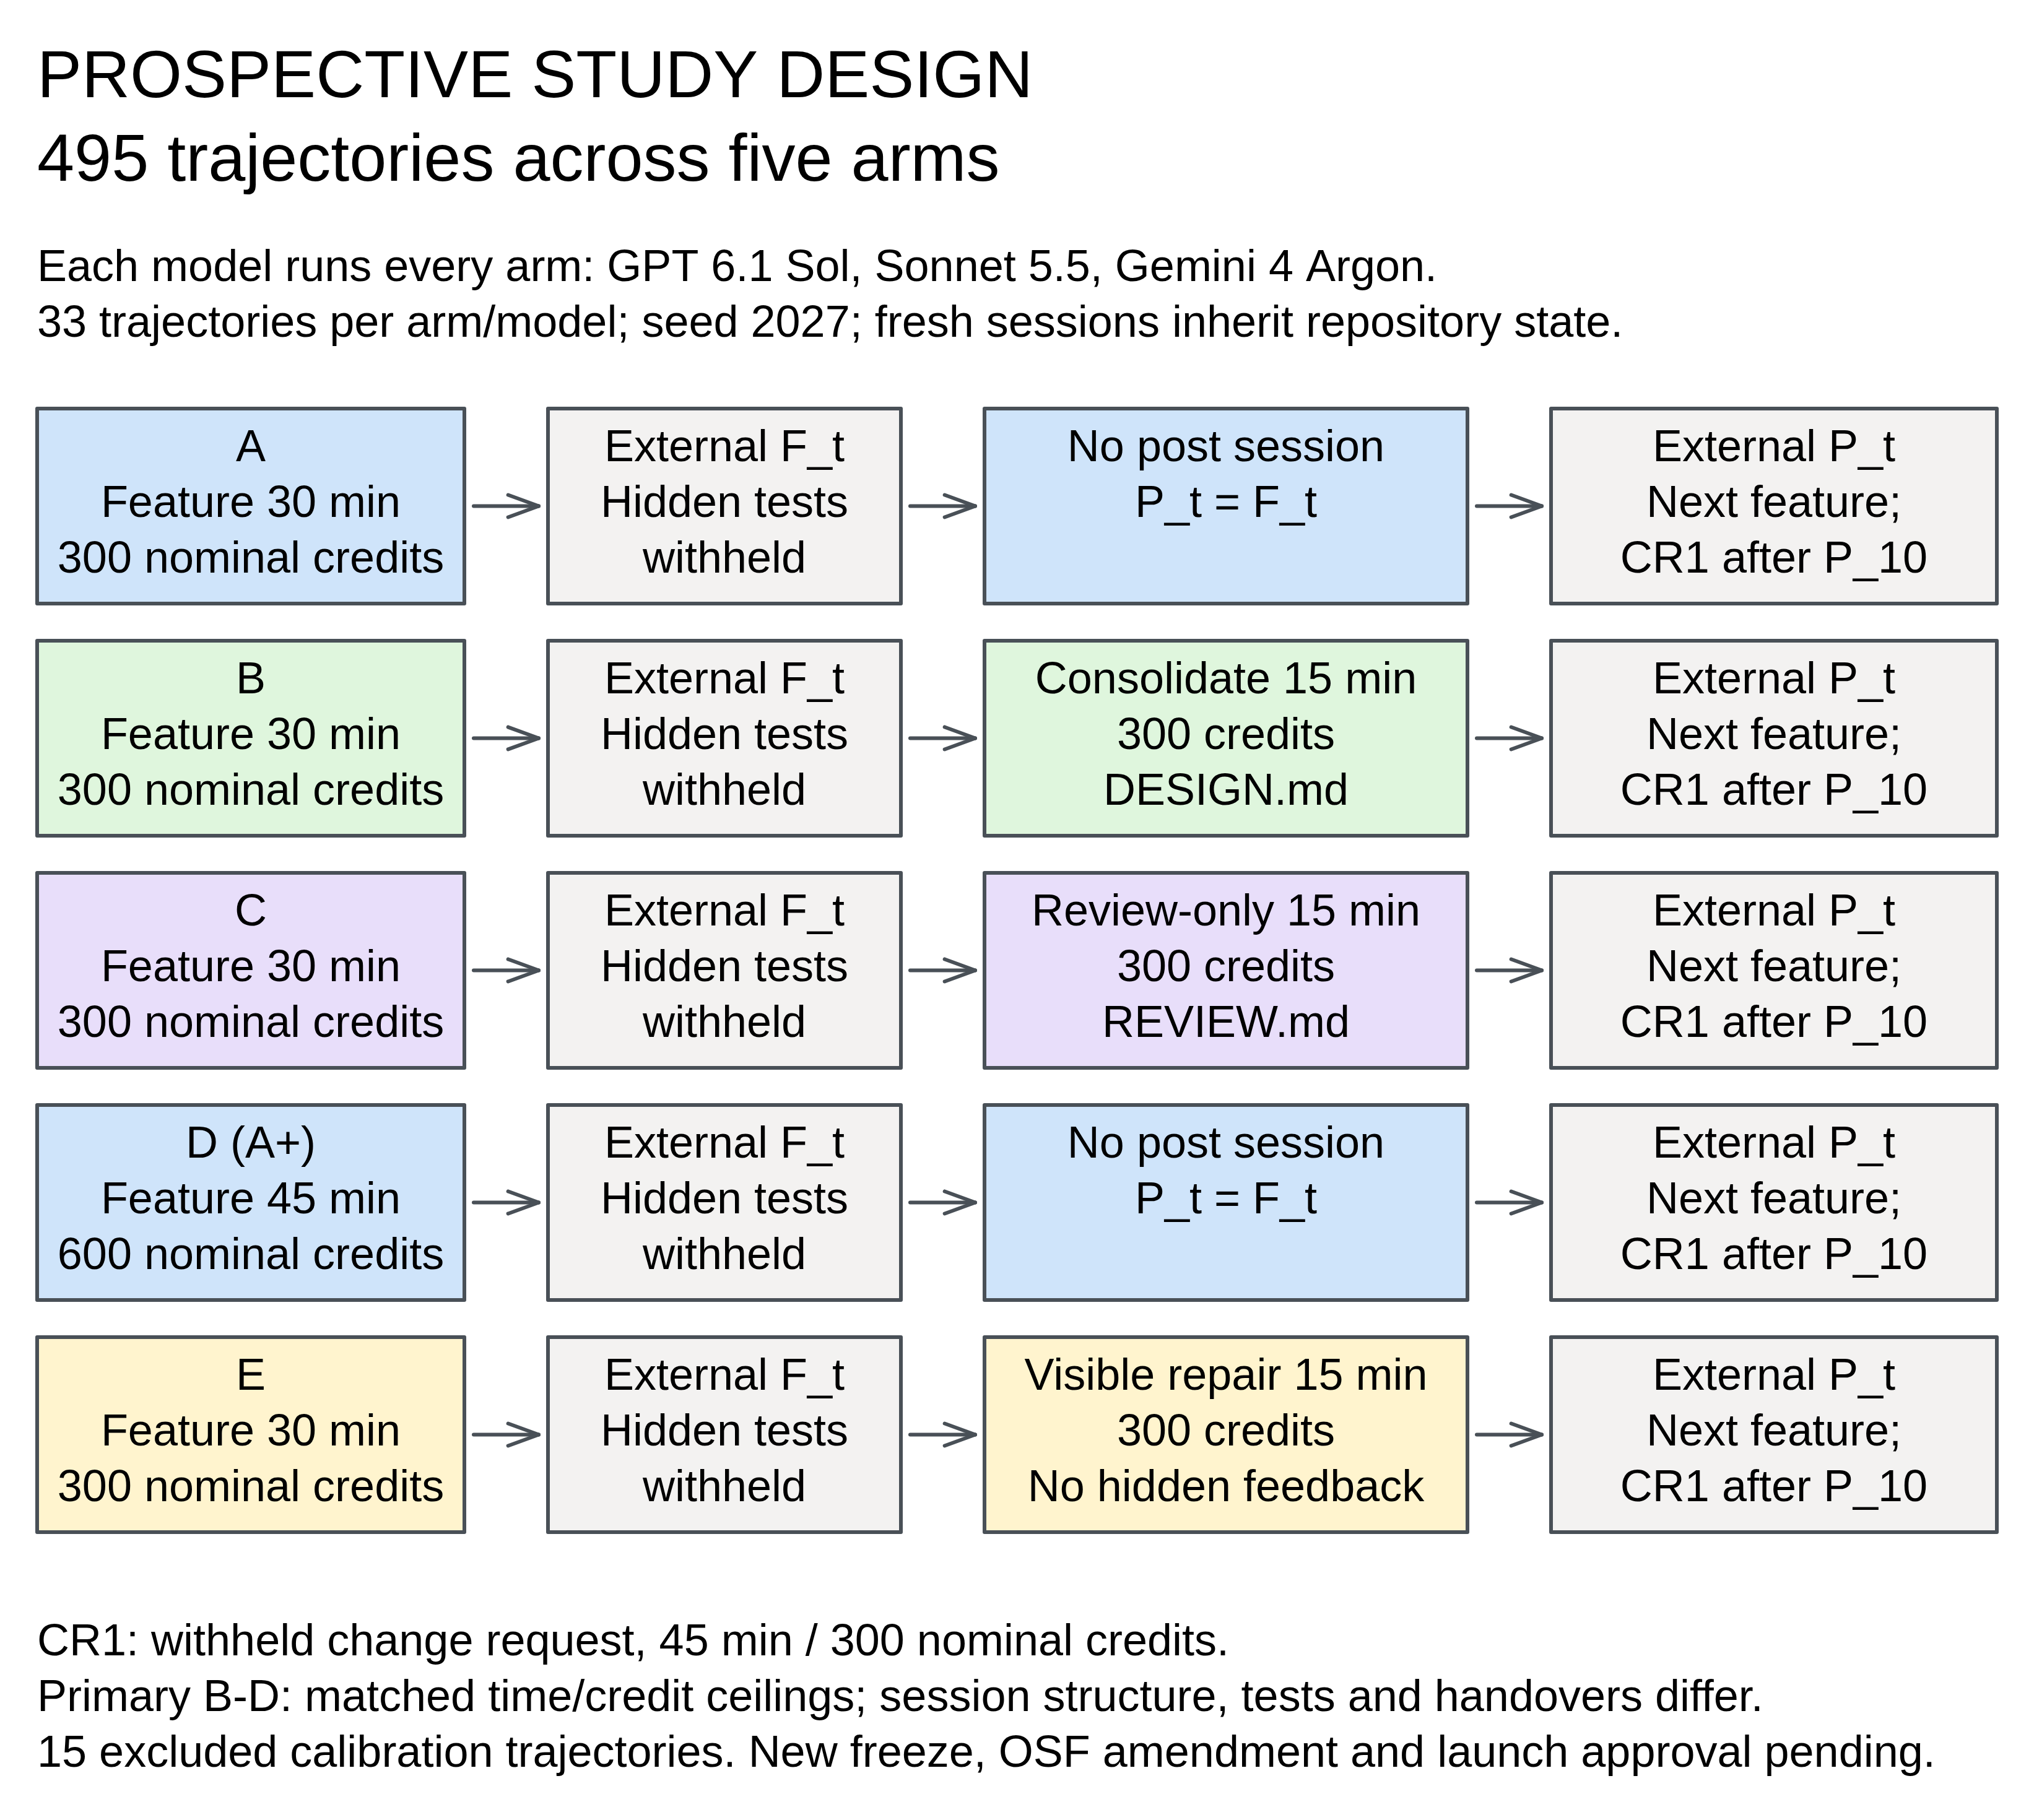
\includegraphics[width=\linewidth]{fig-pilot-design.png}
\caption{Prospective design, not results. Every model runs all five arms.
The external evaluator is separate from candidate tools. CR1 content
remains withheld until its session; privacy and isolation reduce exposure
without proving that a model has no prior knowledge.}\label{fig:pilotdesign}
\end{figure}

\subsection{Outcomes and retained-contract loss}\label{sec:decaymeasurement}

The primary outcome is final behavioural coverage: contracts passed out
of all 127 scheduled feature contracts at $P_{10}$, before CR1.
Coverage combines acquisition, retention and repair.
Retained-contract loss and CR1 adaptation are distinct secondary outcomes,
with legacy identifiers H2 and H6 retained only for data traceability.
HIR/IDR definitions are in the supplementary appendices;
comprehension is not measured.

For trajectory $r$, $F_t$ is the retained state after feature step $t$ and
$P_t$ the state after its assigned post-step; these source states coincide
in A and D. Let $\mathcal{R}_{r,t}$ contain eligible, unchanged contracts
that passed at least one earlier end-of-cycle checkpoint $P_u$, $u<t$.
Superseded contracts leave this risk set. At $F_t$ and $P_t$, let
$\mathcal{O}^{p}_{r,t}\subseteq\mathcal{R}_{r,t}$ contain contracts with
observed binary results $S^p_{r,t}(q)$, $p\in\{F,P\}$. Report
\begin{equation}
L^p_{r,t}=\sum_{q\in\mathcal{O}^{p}_{r,t}}
\mathbf{1}\{S^p_{r,t}(q)=0\},\qquad
d^p_{r,t}=\frac{L^p_{r,t}}{|\mathcal{O}^{p}_{r,t}|}.
\label{eq:decayloss}
\end{equation}
The density is checkpoint prevalence of failure among observed,
previously acquired contracts. An empty observed denominator is undefined.
Publish the full risk set, observed subset and missing count
$M^p_{r,t}=|\mathcal{R}_{r,t}|-|\mathcal{O}^p_{r,t}|$ alongside it.
The full-risk loss count lies between $L^p_{r,t}$ and
$L^p_{r,t}+M^p_{r,t}$; missing evaluations cannot be treated as passes.
Never-acquired contracts remain acquisition failures.
Retain onset, recovery, recurrence and uncertainty across missing
checkpoints. Recovery does not erase an episode. Distinguish same-cycle
post-step losses and rejected attempts from losses in retained code.

\begin{figure}[!htbp]
\centering
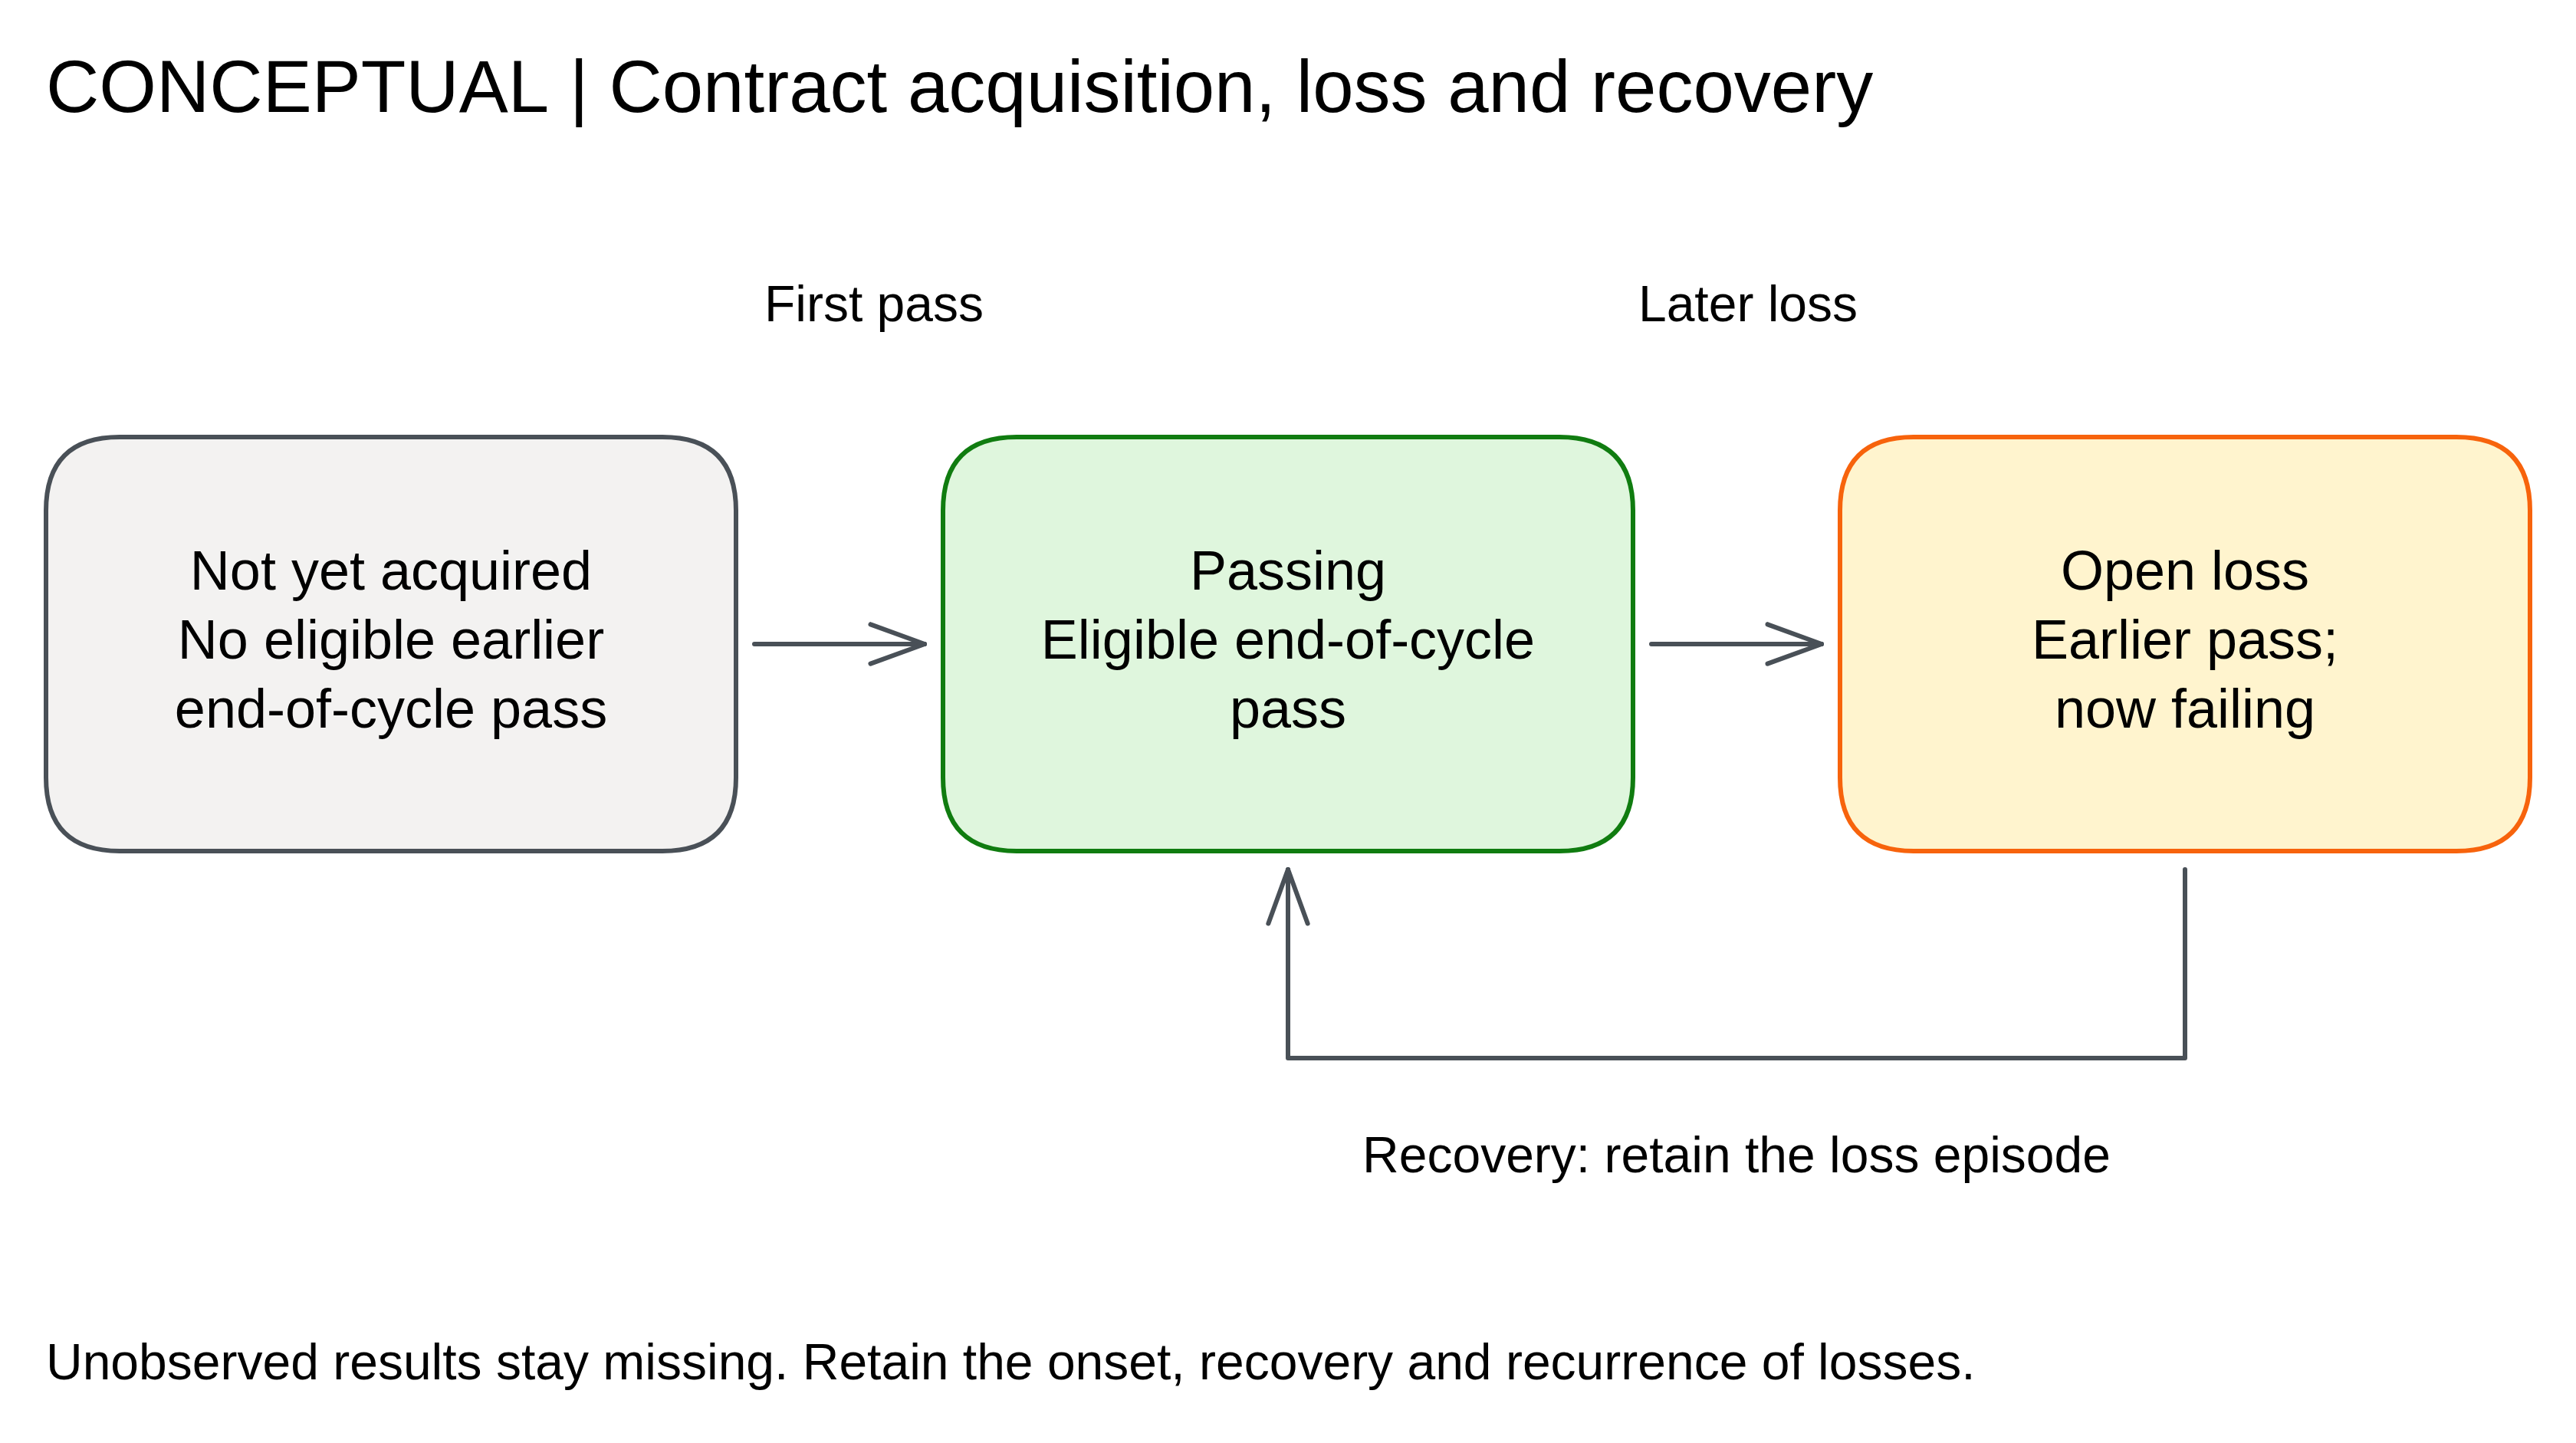
\includegraphics[width=\linewidth]{fig-contract-states.png}
\caption{Conceptual contract states. Acquisition, loss, recovery and
unobserved evaluation are distinct; the diagram contains no measured
frequencies.}\label{fig:contractstates}
\end{figure}

CR1 success requires all 15 CR1 contracts and retention of every feature
contract passing before CR1. Also report contracts passed out of 15,
previously passing contracts lost, and observed/missing denominators.
Stratify by whether F9 and F10 prerequisites were acquired before CR1:
an incomplete arm has fewer retention obligations, and prerequisite
strata are post-treatment selections, not randomised subgroups.
One fixed CR1 is task-specific. A prewritten, randomly selected request
pool belongs to a separately registered subsequent study.

\begin{figure}[!htbp]
\centering
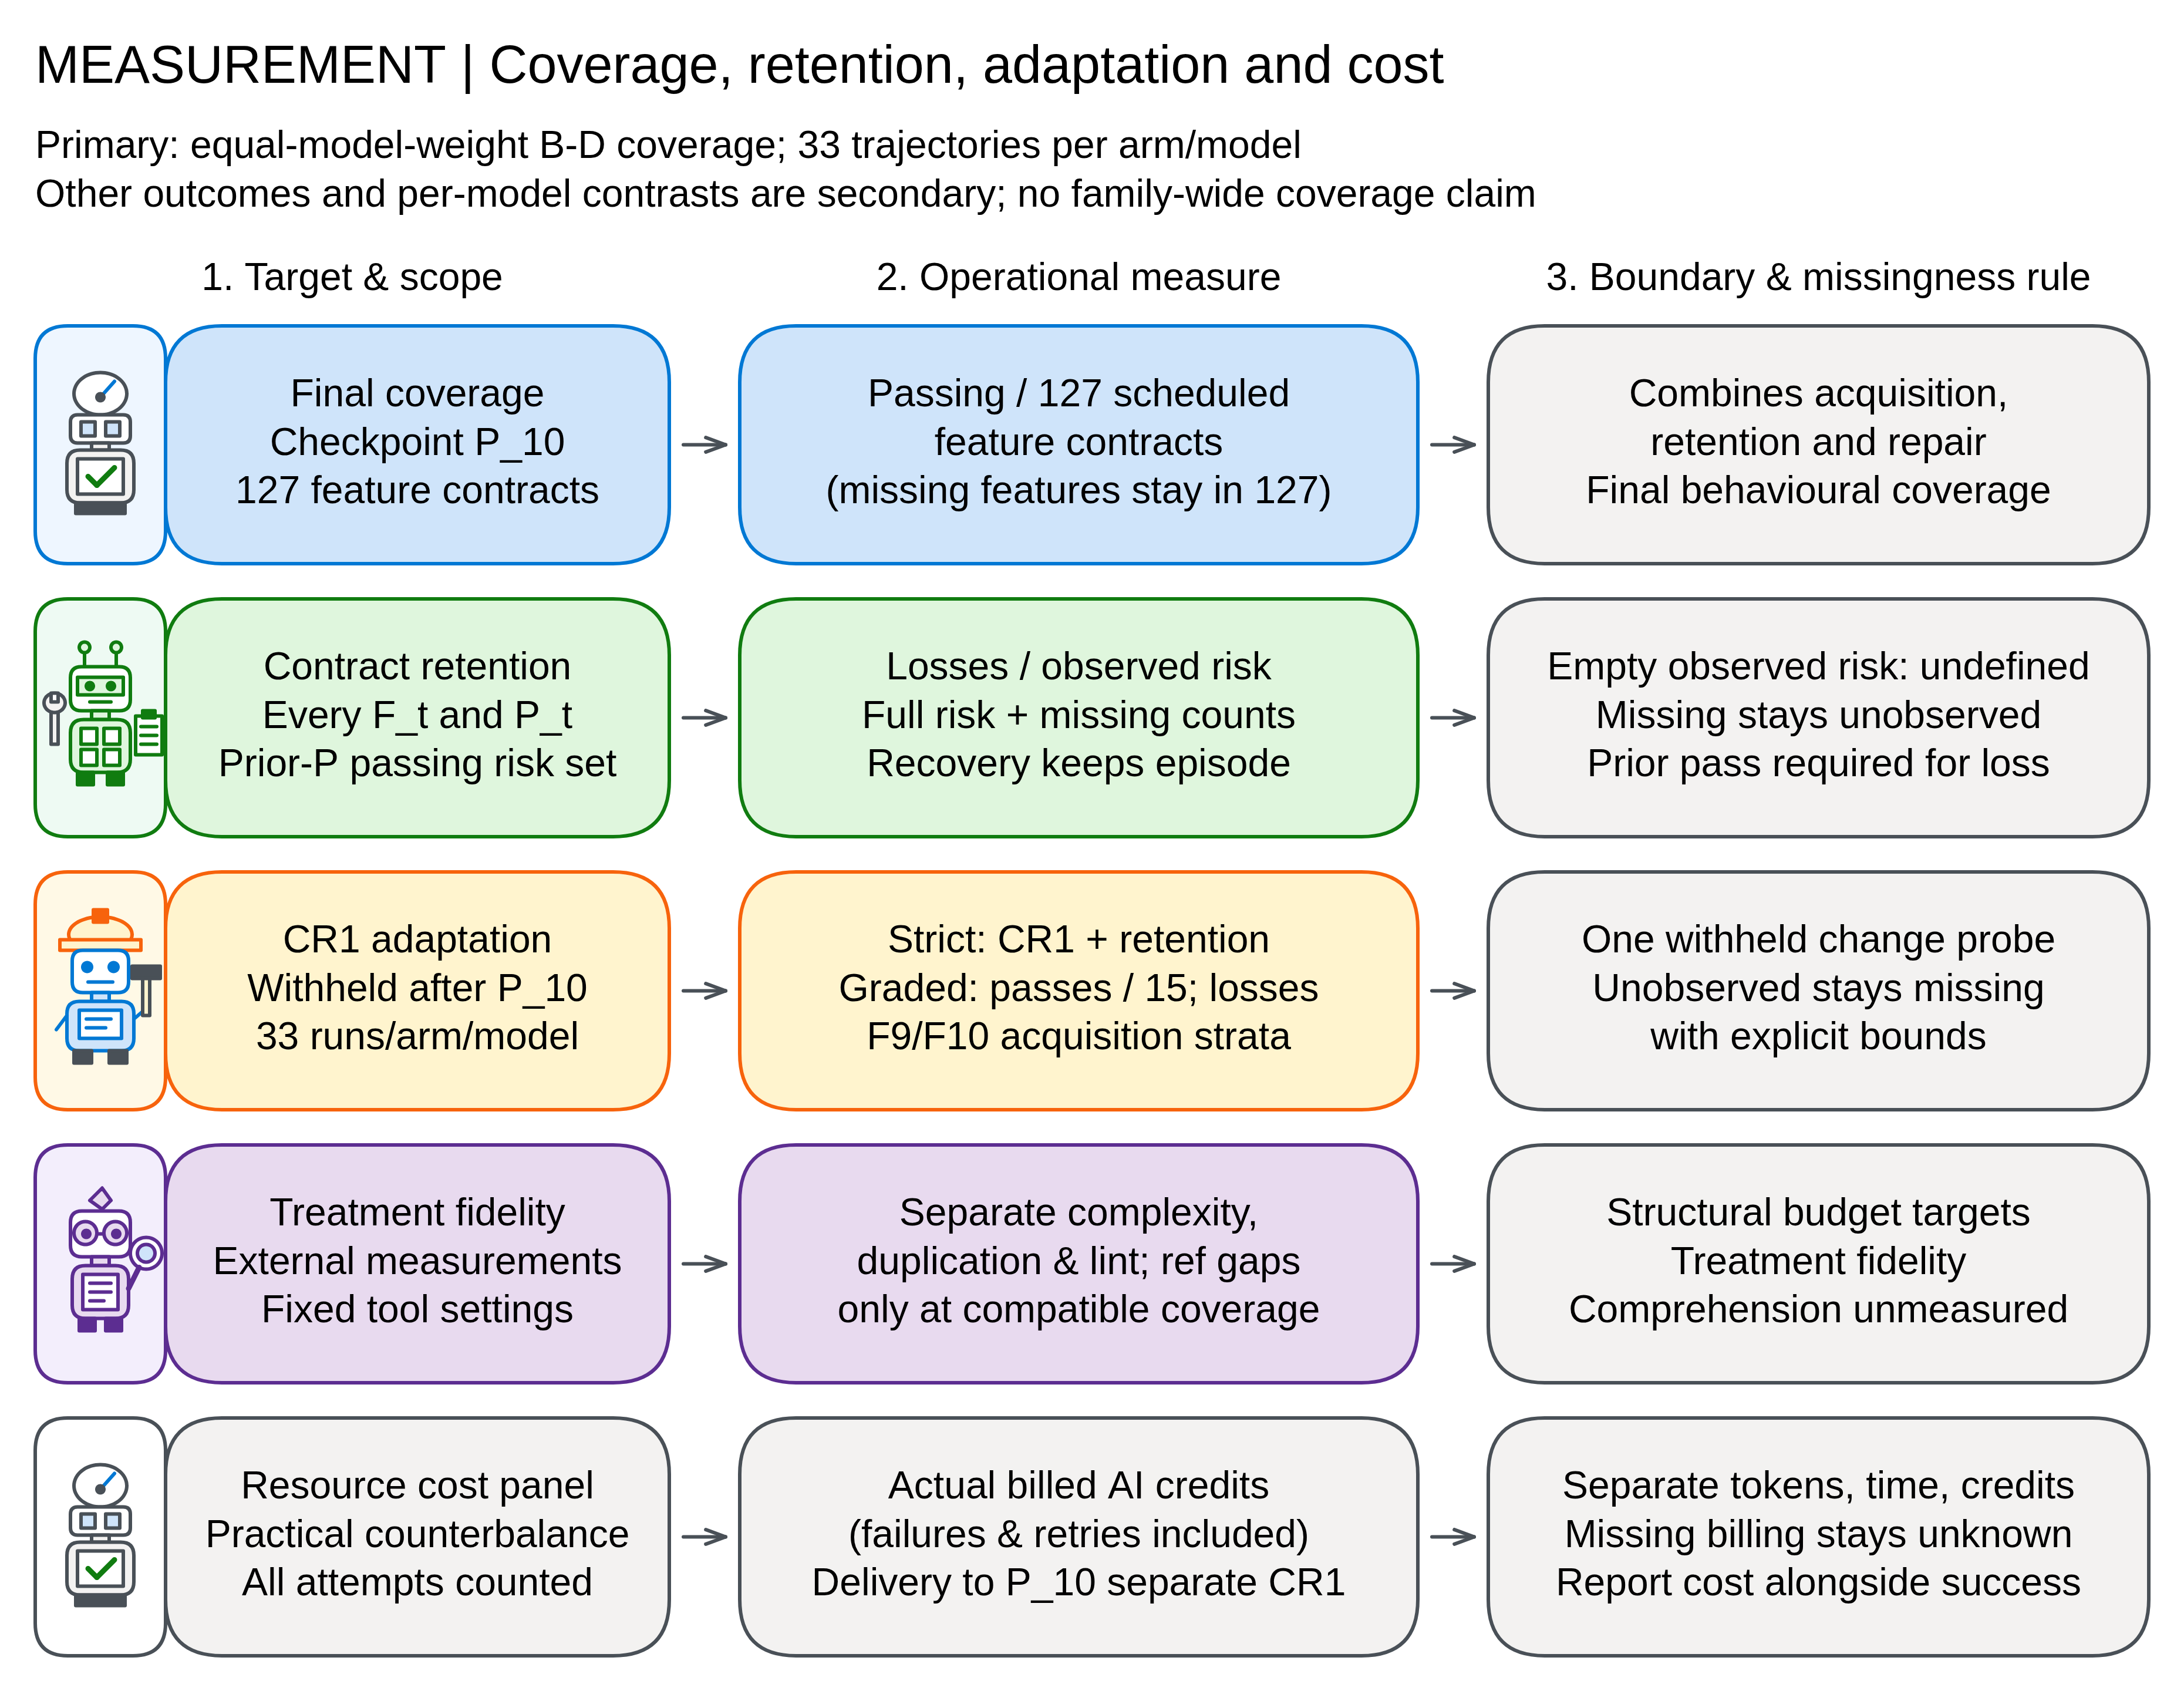
\includegraphics[width=\linewidth]{fig-experiment-measures.png}
\caption{Coverage, retained behaviour, adaptation and all-attempt cost
are separate measures. Structural metrics targeted by B's stopping
budget are treatment-fidelity checks, not independent efficacy outcomes.
Unknown results and billing remain unknown.}\label{fig:experimentmeasures}
\end{figure}

Actual AI credits include every delivery and CR1 attempt, including
failures, assistance and infrastructure retries; phases are reported
separately. Cheap failure is not efficiency. Credits, tokens, elapsed
time and currency are distinct. Lizard measures complexity, Ruff lint
and jscpd duplication. External fixed settings and
\texttt{ruff --isolated --ignore-noqa} prevent local suppressions from
silently improving the lint score; count added suppressions separately.
SDK request wall time and tool time are observable. Provider-active
time and rate-limit waits require explicit telemetry; absent telemetry
is not zero.

\subsection{Replication and uncertainty}\label{sec:protocollimits}

The author selected a minimum useful absolute coverage gain of ten
percentage points, approximately thirteen test-weighted contracts.
Coverage scores $Y$ are expressed on the 0--100 scale. Let
$\overline{Y}_{ma}$ be mean final coverage for model $m$ and arm $a$.
The primary estimand is the equal-model-weight difference in mean coverage
over the $M=3$ selected models. Its estimator is
\begin{equation}
\widehat{\Delta}_{BD}=\frac{1}{M}
\sum_{m=1}^{M}(\overline{Y}_{mB}-\overline{Y}_{mD}).
\label{eq:primarycontrast}
\end{equation}
For balanced cells of $n_{\mathrm{cell}}$ independent trajectories and a
common within-cell variance $\sigma^2$, its planning variance is
$2\sigma^2/(M n_{\mathrm{cell}})$. The assumed SD is 25 percentage points.
For one two-sided comparison with $\alpha=0.05$, target power
$1-\beta=0.80$ and target difference $\Delta_*=10$ points, the normal
planning approximation is
\begin{equation}
n_{\mathrm{cell}}=
\left\lceil\frac{2(z_{1-\alpha/2}+z_{1-\beta})^2\sigma^2}
{M\Delta_*^2}\right\rceil=33.
\label{eq:samplesize}
\end{equation}
This gives 99 trajectories per arm, 495 overall. The target power is
conditional on independent trajectories, the assumed variance and the
blocked estimand; it is not guaranteed. SD assumptions of 15, 20 and
50 points require 12, 21 and 131 per cell respectively. The bounded
score's worst-case SD is 50; the 25-point assumption needs explicit
author and prospective registration approval.

Resample whole trajectories within model and arm, with
10,000 draws and pointwise 95\% percentile intervals; disclose missing
frames rather than silently pool observed models or complete cases.
Model-specific estimates and other contrasts are secondary, with no
family-wide coverage claim.
Retain scheduling-block identifiers. Before collection, source-bound review
must reconcile this independent-trajectory variance and bootstrap scheme
with the model/replicate blocking: residual dependence would require a
block-preserving analysis and revised planning variance.
% TODO(author): resolve scheduling-block dependence and bind the variance/resampling choice to the new kit freeze and prospective registration.
Chen, Zaharia and Zou's dated ChatGPT comparison motivates monitoring
service drift despite exposed names~\cite{chen2023drift}; it does not
measure drift in this roster or make a version pin an immutability guarantee.
Report the pooled within-cell SD with its
degrees of freedom for future planning.
For binary CR1, report per-model success counts and exact binomial
component intervals under independent runs with a common success
probability within each cell. Aggregate contrasts must preserve model
strata. The coverage calculation supplies no power guarantee for CR1.

\subsection{Resources, feasibility and collection gates}\label{sec:prerun}

The unchanged envelope is 300,000 nominal credits, with 270,000 local
admission, prior spending and unknown historical provisions retained.
Original 300-credit sessions use a 270-credit soft limit; D's
600-credit feature uses 540. A retry shares the original allowance.
In-flight responses can overshoot; these are not provider billing caps.
No verified dollar conversion is available.

\begin{table}[!htbp]
\centering\small
\caption{Planned resources, not expenditure. Worst-case allowances
exceed the aggregate envelope; affordability is a real launch gate.}
\label{tab:pilotresources}
\begin{tabular}{@{}lrrr@{}}
\toprule
Arm & Trajectories & Sessions & Maximum agent-hours \\
\midrule
A & 99 & 1,089 & 569.25 \\
B & 99 & 2,079 & 816.75 \\
C & 99 & 2,079 & 816.75 \\
D & 99 & 1,089 & 816.75 \\
E & 99 & 2,079 & 816.75 \\
Study total & 495 & 8,415 & 3,836.25 \\
Excluded calibration, no CR1 & 15 & 240 & 105.00 \\
\bottomrule
\end{tabular}
\end{table}

At nominal caps the combined allowance is 2,902,500 credits, not a
permitted expenditure. Cost-only excluded calibration must show that
the entire fixed allocation fits remaining admission and the deadline;
otherwise halt and amend before collection, never quietly reduce the
sample. Proposed progression criteria are infrastructure failures at
most 5\%, no missing primary observations, complete billing/model/help
records, zero oracle contradictions in triplicate reference checks,
and no information-boundary failure. Hidden-test mutation assessment
must report its actual mutant denominator and unresolved equivalence.
These are feasibility criteria, inspired by pilot-study guidance
~\cite{eldridge2016pilot}, not a clinical CONSORT compliance claim.

Only current and previous visible specifications and examples reach
candidate tools. Hidden tests, scores, identifiers, messages, reference
code and future CR1 remain external. Candidate commands use no-network
containers; the trusted host SDK's provider connection is different.
The independent researcher receives a protected kit without access to
the original repositories or manuscript.
Use a researcher-managed workspace/account without the author's original
checkouts, manuscript or session-context caches; record actual access and
prior exposure rather than assuming blindness from a private flag.
The owner will make both
repositories private before collection and release approved materials
with the paper afterward. OSF registration/embargo and GitHub privacy
are separate; neither removes prior public or model exposure.
Fresh source-bound access checks, approval, freeze, prospective OSF
recording and launch permission remain required.

Unsuccessful feature increments are reset; later features and scheduled
B/C/E post-steps continue on retained green state. Hidden denominators
still include undelivered features. One infrastructure-only retry shares
the original budget; poor performance never justifies replay.
Contradictory valid oracle results halt collection.
Assisted and incomplete trajectories and all their costs are retained,
without replacements or success-conditioned primary analyses.

\ifresults
% TODO(author): insert the prospectively collected results and checked analysis.
\else
% TODO(author): PF1 requires actual F/P checkpoint vectors, eligibility and missingness.
% TODO(author): PF2 requires actual CR1 vectors, prerequisites, assistance and all-attempt costs.
% TODO(author): PF3 requires actual final coverage and attributable delivery credits.
\fi
